\documentclass{article}

\usepackage{graphicx}
\usepackage{amssymb}
\usepackage{lastpage}
\usepackage{epstopdf}
\usepackage{fancyhdr}
\DeclareGraphicsRule{.tif}{png}{.png}{`convert #1 `dirname #1`/`basename #1 .tif`.png}
\usepackage{titling}
\setlength{\droptitle}{-1.2in}

\newcommand{\cTitle}{NYU ICPC Team Codebook}
\newcommand{\cAuthor}{Compiled for the 2012 GNYR}
\usepackage[margin=3cm]{geometry}
\pagestyle{fancy}
\lhead{\cAuthor}                                                 %
\rhead{\cTitle}  %
\lfoot{\lastxmark}                                                      %
\cfoot{}                                                                %
\rfoot{Page\ \thepage\ of\ \pageref{LastPage}}                          %
\renewcommand\headrulewidth{0.4pt}                                      %
\renewcommand\footrulewidth{0.4pt}        
\hfuzz=96pt

\title{\cTitle}
\author{\cAuthor}
\begin{document}
\maketitle


This collaborative document is the central place for the algorithms you will need for the ACM ICPC programming contest.

\tableofcontents

%Codebook wishlist:

%Minimum weighted bipartite matching
%Chinese remainder theorem
%Matrix operations
%Floyd-Warshall's shortest path

\clearpage
\section*{The Ritual}
\addcontentsline{toc}{section}{The Ritual}

\subsection*{When Choosing a Problem}

* Find out which balloons are the popular ones!
* Pick one with a nice, clean solution that you are totally convinced
will work to do first.

\subsection*{Before Designing Your Solution}

* Highlight the important information on the problem statement - input
bounds, special rules, formatting, etc.
* Look for code in this notebook that you can use!
* Convince yourself that your algorithm will run with time to spare on
the biggest input.
* Create several test cases that you will use, especially for special
or boundary cases.

\subsection*{Prior to Submitting}

* Check maximum input, zero input, and other degenerate test cases.
* Cross check with team mates' supplementary test cases.
* Read the problem output specification one more time - your program's
output behaviour is fresh in your mind.
* Does your program work with negative numbers?
* Make sure that your program is reading from an appropriate input file.
* Check all variable initialisation, array bounds, and loop variables
(i vs j, m vs n, etc.).
* Finally, run a diff on the provided sample output and your program's output.
* And don't forget to submit your solution under the correct problem number!

\subsection*{After Submitting}

* Immediately print a copy of your source.
* Staple the solution to the problem statement and keep them safe.  Do
not lose them!

\subsection*{If It Doesn't Work...}

* Remember that a run-time error can be division by zero.
* If the solution is not complex, allow a team mate to start the
problem afresh.
* Don't waste a lot of time - it's not shameful to simply give up!!!

\clearpage
\section*{Skeleton File}
\addcontentsline{toc}{section}{Skeleton File}
\begin{verbatim}
//COMPILING & RUNNING: javac Main.java && java Main < input.txt 

import java.util.*;

public class Main {

    public static Scanner in;
 
    public static void main(String[] args) {
        in = new Scanner(System.in);

        doStuff();
    }

    public static void doStuff() {
        int N = in.nextInt();

        for(int i = 0;i < N; i++) {
            solve();
        }
    }

    public static void solve() {

    }
}
\end{verbatim}
\clearpage
\section*{Geometry}
\addcontentsline{toc}{section}{Geometry}
\addcontentsline{toc}{subsection}{Points and Polygons}
\begin{verbatim}
/*
 * PtD - Point class 
 * Required for most of the geometric algorithms below.
 * convex hull, 3 point circle,
 * intersection of circles, centroid/area of a polygon
 * @author Darko Aleksic
 */
class PtD {
  public static final double EPS = 1e-9;
  double x, y;

  /* add hashCode() and equals() if needed */
  PtD(double x, double y) {
    this.x = x;
    this.y = y;
  }

  public double dist(PtD p) {
    return Math.sqrt(distSquared(p));
  }

  public double distSquared(PtD p) {
    double dx = x - p.x;
    double dy = y - p.y;
    return dx * dx + dy * dy;
  }

  // For debugging.
  public String toString(){
    return "(" + x + "," + y + ")";
  }

  public int compareTo(PtD p2) {
    if (Math.abs(y - p2.y) < EPS) {
      if (Math.abs(x - p2.x) < EPS)
        return 0;
      if (x < p2.x)
        return -1;
      return 1;
    }
    if (y < p2.y)
      return -1;
    return 1;
  }

  public int compareTo(PtD p2, PtD pivot) {
    if (Math.abs(y - pivot.y) < EPS && Math.abs(y - p2.y) < EPS) {
      if (Math.abs(x - p2.x) < EPS)
        return 0;
      if (x > p2.x) // !!
        return -1;
      return 1;
    }
    double k = sub(pivot).cross(p2.sub(pivot));
    if (Math.abs(k) < EPS) {
      double d = distSquared(pivot) - p2.distSquared(pivot);
      if (Math.abs(d) < EPS)
        return 0;
      if (d < 0)
        return -1;
      return 1;
    }
    if (k < 0)
      return -1;
    return 1;
  }

  public PtD sub(PtD p2) {
    return new PtD(x - p2.x, y - p2.y);
  }

  public double dot(PtD p2) {
    return x * p2.x + y * p2.y;
  }

  public double cross(PtD p2) {
    return x * p2.y - p2.x * y;
  }
    \end{verbatim}
\addcontentsline{toc}{subsubsection}{Centroid}
  \begin{verbatim}
  /* centroid - they must be in order 
   * (CW or CCW, does not matter)
   */
  public static PtD centroid(PtD[] p, int n) {
    PtD c = new PtD(0, 0);
    int i, j;
    double sum = 0;
    double area = 0;
    for (i = n - 1, j = 0; j < n; i = j++) {
      area = p[i].x * p[j].y - p[i].y * p[j].x;
      sum += area;
      c.x += (p[i].x + p[j].x) * area;
      c.y += (p[i].y + p[j].y) * area;
    }
    sum *= 3.0;
    c.x /= sum;
    c.y /= sum;
    return c;
  }

    \end{verbatim}
\addcontentsline{toc}{subsubsection}{Signed Area}
    \begin{verbatim}
  /* signed area of a polygon */
  public static double signedArea(PtD[] p, int n) {
    double sum = 0;
    for (int i = n - 1, j = 0; j < n; i = j++) {
      sum += p[i].x * p[j].y - p[i].y * p[j].x;
    }
    return 0.5 * sum;
  }

    \end{verbatim}
\addcontentsline{toc}{subsubsection}{Circle through three points}
  \begin{verbatim}
  /**
   * Circle through three points
   * 
   * @return a[]={x,y,r}, null if colinear
   */
  public static double[] circleThroughThreePoints(PtD A, PtD B, PtD C) {
    double[] a = new double[3];
    double area = 0.5 * ((B.x - A.x) * (C.y - A.y) - (C.x - A.x)
        * (B.y - A.y));
    if (Math.abs(area) < EPS)
      return null;
    double lbaSqr = (B.x - A.x) * (B.x - A.x) + (B.y - A.y) * (B.y - A.y);
    double lcaSqr = (C.x - A.x) * (C.x - A.x) + (C.y - A.y) * (C.y - A.y);
    a[0] = A.x + ((C.y - A.y) * lbaSqr - ((B.y - A.y) * lcaSqr))
        / (4 * area);
    a[1] = A.y + ((B.x - A.x) * lcaSqr - ((C.x - A.x) * lbaSqr))
        / (4 * area);
    a[2] = Math.sqrt((a[0] - A.x) * (a[0] - A.x) + (a[1] - A.y)
        * (a[1] - A.y));
    return a;
  }

    \end{verbatim}
\addcontentsline{toc}{subsubsection}{Intersection of Circles}
  \begin{verbatim}
  /**
   * Intersection of circles. PtD needs sub[traction](), dot() and EPS defined
   * 
   * @param p0
   *      Center of 1st circle
   * @param p1
   *      Center of 2nd circle
   * @param r0
   *      radius of 1st circle
   * @param r1
   *      radius of 2nd circle
   * @param a
   *      array that will hold the points (if any)
   * @return number of intersection points (-1 means infinity)
   */
  public static int circleIntersection(PtD p0, PtD p1, double r0, double r1,
      PtD[] a) {
    PtD U = p1.sub(p0);
    PtD V = new PtD(U.y, -U.x);
    double duSqr = U.dot(U);
    double du = Math.sqrt(duSqr);
    if (Math.abs(U.x) < EPS && Math.abs(U.y) < EPS
        && Math.abs(r0 - r1) < EPS) {
      return -1; // same circles
    }
    if (Math.abs(du - (r0 + r1)) < EPS) {
      // one point from outside
      double cc = r0 / (r0 + r1);
      a[0] = new PtD(p0.x + cc * U.x, p0.y + cc * U.y);
      return 1;
    }
    if (Math.abs(du - Math.abs(r0 - r1)) < EPS) {
      // one point from inside
      double cc = r0 / (r0 - r1);
      a[0] = new PtD(p0.x + cc * U.x, p0.y + cc * U.y);
      return 1;
    }
    if (du - Math.abs(r0 - r1) >= EPS && (r0 + r1) - du >= EPS) {
      // two points
      double s = 0.5 * ((r0 * r0 - r1 * r1) / duSqr + 1);
      double t = Math.sqrt(r0 * r0 / duSqr - s * s);
      a[0] = new PtD(p0.x + s * U.x + t * V.x, p0.y + s * U.y + t * V.y);
      a[1] = new PtD(p0.x + s * U.x - t * V.x, p0.y + s * U.y - t * V.y);
      return 2;
    }
    // no intersection
    return 0;
  }

    \end{verbatim}
\addcontentsline{toc}{subsubsection}{Graham Scan (Convex Hull)}
    \begin{verbatim}
    /**
     * @param ps
     *            array containing the set of distinct points
     * @param n
     *            number of points
     * @return array of points on the convex hull (may be empty, if n<=0)
     */
    public static PtD[] grahamScan(PtD[] ps, int n, boolean keepColinear) {
        // maybe check for these outside?
        if (n <= 0) {
            PtD[] ret = new PtD[0];
            return ret; // or null?
        }
        if (n == 1) {
            PtD[] ret = new PtD[1];
            ret[0] = ps[0];
            return ret;
        }
        // find pivot and sort
        int p = 0;
        for (int i = 1; i < n; i++) {
            if (ps[i].compareTo(ps[p]) < 0)
                p = i;
        }
        PtD tmp = ps[0];
        ps[0] = ps[p];
        ps[p] = tmp;
        angularSort(ps, 1, n);
        // check if they are all on the same line
        if (Math.abs((ps[n - 1].sub(ps[0])).cross(ps[1].sub(ps[0]))) < EPS) {
            if (keepColinear) {
                PtD[] ret = new PtD[n];
                ret[0] = ps[0];
                if (ps[0].distSquared(ps[1]) >= ps[0].distSquared(ps[n - 1])
                        + EPS)
                    for (int i = 1; i < n; i++)
                        ret[n - i] = ps[i];
                else
                    for (int i = 1; i < n; i++)
                        ret[i] = ps[i];
                return ret;
            } else {
                PtD[] ret = new PtD[2];
                ret[0] = ps[0];
                if (ps[0].distSquared(ps[1]) >= ps[0].distSquared(ps[n - 1])
                        + EPS)
                    ret[1] = ps[1];
                else
                    ret[1] = ps[n - 1];
                return ret;
            }
        }
        // remove closer ones on the same line
        PtD[] tps = new PtD[n];
        tps[0] = ps[0];
        tps[1] = ps[1];
        int tt = 0;
        int start = 2;
        int end = n;
        if (keepColinear) {
            PtD a = ps[0].sub(ps[1]);
            while (Math.abs(a.cross(ps[0].sub(ps[start]))) < EPS) {
                tps[start] = ps[start];
                start++;
            }
            a = ps[0].sub(ps[n - 1]);
            while (Math.abs(a.cross(ps[0].sub(ps[end - 1]))) < EPS) {
                end--;
            }
            end++;
        }
        for (int i = start; i < end; i++) {
            PtD a = tps[i - tt - 1].sub(tps[i - tt - 2]);
            PtD b = ps[i].sub(tps[i - tt - 2]);
            if (!keepColinear && Math.abs(a.cross(b)) < EPS) {
                tps[i - tt - 1] = ps[i];
                tt++;
            } else {
                tps[i - tt] = ps[i];
            }
        }
        for (int i = end; i < n; i++) {
            tps[i - tt] = ps[i];
        }
        // remove last point if colinear
        if (!keepColinear && n - tt > 2) {
            PtD a = tps[0].sub(tps[n - tt - 2]);
            PtD b = tps[0].sub(tps[n - tt - 1]);
            if (Math.abs(a.cross(b)) < EPS)
                tt++;
        }
        n -= tt;
        PtD[] stack = new PtD[n];
        int stackSize = 0;
        stack[stackSize++] = tps[0];
        stack[stackSize++] = tps[1];
        for (int i = 2; i < n; i++) {
            while (true) {
                PtD a = stack[stackSize - 1].sub(stack[stackSize - 2]);
                PtD b = tps[i].sub(stack[stackSize - 2]);
                double cross = a.cross(b);
                if (cross <= -EPS || (cross < EPS && keepColinear))
                    break;
                stackSize--;
            }
            stack[stackSize++] = tps[i];
        }
        PtD[] ret = new PtD[stackSize];
        System.arraycopy(stack, 0, ret, 0, stackSize);
        return ret;
    }

    \end{verbatim}
\addcontentsline{toc}{subsubsection}{Angular Sort}
    \begin{verbatim}
    private static void angularSort(PtD ps[], int begin, int end) {
        int mid;
        if (end - begin <= 1) {
            return;
        }
        mid = (begin + end) / 2;
        angularSort(ps, begin, mid);
        angularSort(ps, mid, end);
        merge(ps, begin, mid, end);
    }

    private static void merge(PtD[] ps, int start, int mid, int end) {
        int i = start;
        int j = mid;
        int k = 0;
        PtD[] temp = new PtD[end - start];
        while ((i < mid) && (j < end))
            if (ps[i].compareTo(ps[j], ps[0]) <= 0) {
                temp[k++] = ps[i++];
            } else {
                temp[k++] = ps[j++];
            }
        while (i < mid) {
            temp[k++] = ps[i++];
        }
        while (j < end) {
            temp[k++] = ps[j++];
        }
        for (i = start; i < end; i++)
            ps[i] = temp[i - start];
    }

}

    \end{verbatim}
\addcontentsline{toc}{subsection}{Segments}
    \begin{verbatim}
/*
 * Seg - segment/ray/line class (distances/intersections)
 * @author Darko Aleksic
 */
class Seg { // needs PtD (not all of it, add as needed)
    double a, b, c; // line ax + by = c
    PtD P0, P1;
    PtD N; // normal, line is nX=c, X=(x,y)
    PtD D; // dir vector, line is P0+tD

    // if it's a ray, pass endpoint as P0
    public Seg(PtD P0, PtD P1) {
        this.P0 = P0;
        this.P1 = P1;
        a = P1.y - P0.y;
        b = P0.x - P1.x;
        c = a * P0.x + b * P0.y;
        // careful with zero-length segments!
        // normalize it?
        double d = P0.dist(P1);
        if (d > PtD.EPS) {
            a /= d;
            b /= d;
            c /= d;
        }
        N = new PtD(a, b);
        D = new PtD(b, -a);
    }

    \end{verbatim}
\addcontentsline{toc}{subsubsection}{Point-(Seg|Line|Ray) Distance}
    \begin{verbatim}
    // generic point-to-segment, can be adjusted to p-to-line or p-to-ray
    public static double squaredDistance(PtD Y, Seg S) {
        PtD DD = S.P1.sub(S.P0);
        PtD YmP0 = Y.sub(S.P0);
        double t = DD.dot(YmP0);
        if (t <= PtD.EPS) // remove if line!
            return YmP0.dot(YmP0);
        double ddd = DD.dot(DD);
        if (t >= ddd - PtD.EPS) { // remove if line OR ray!
            PtD YmP1 = Y.sub(S.P1);
            return YmP1.dot(YmP1);
        }
        return YmP0.dot(YmP0) - t * t / ddd; // maybe abs() if 0.0?
    }

    \end{verbatim}
\addcontentsline{toc}{subsubsection}{Line-Line Distance}
    \begin{verbatim}
    public static double lineToLineDistance(Seg line1, Seg line2) {
        double cross = line1.N.dot(line2.D);
        if (Math.abs(cross) >= PtD.EPS)
            return 0;// they intersect
        double dot = line1.N.dot(line2.N);
        if (dot < 0) // fishy? but if close to 0, does not matter?
            return Math.abs(line2.c + line1.c);
        else
            return Math.abs(line2.c - line1.c);
    }

    \end{verbatim}
\addcontentsline{toc}{subsubsection}{Line-Seg Distance}
    \begin{verbatim}
    public static double lineToSegmentDistance(Seg line, Seg segment) {
        double q0 = line.N.dot(segment.P0) - line.c;
        double q1 = line.N.dot(segment.P1) - line.c;
        if (q0 * q1 <= -PtD.EPS)
            return 0;
        return Math.min(Math.abs(q0), Math.abs(q1));
    }

    \end{verbatim}
\addcontentsline{toc}{subsubsection}{Seg-Seg Distance}
    \begin{verbatim}
    public static double segmentToSegmentDistance(Seg seg1, Seg seg2) {
        if (overlap(seg1, seg2) != null)
            return 0;
        if (isect(seg1, seg2) != null)
            return 0;
        double d = squaredDistance(seg1.P0, seg2);
        d = Math.min(d, squaredDistance(seg1.P1, seg2));
        d = Math.min(d, squaredDistance(seg2.P0, seg1));
        return Math.sqrt(Math.min(d, squaredDistance(seg2.P1, seg1)));
    }

    public boolean contains(PtD p) {
        return Math.abs(a * p.x + b * p.y - c) < PtD.EPS
                && Math.min(P0.x, P1.x) - PtD.EPS <= p.x
                && p.x <= Math.max(P0.x, P1.x) + PtD.EPS
                && Math.min(P0.y, P1.y) - PtD.EPS <= p.y
                && p.y <= Math.max(P0.y, P1.y) + PtD.EPS;
    }

    \end{verbatim}
\addcontentsline{toc}{subsubsection}{Seg-Seg Intersection}
    \begin{verbatim}
    public static PtD isect(Seg s, Seg t) {
        double d = s.a * t.b - s.b * t.a;
        if (Math.abs(d) < PtD.EPS)
            return null; // parallel lines, deal with them somewhere else
        PtD p = new PtD((s.c * t.b - s.b * t.c) / d, (s.a * t.c - s.c * t.a)
                / d);
        if (!s.contains(p) || !t.contains(p))
            return null;
        return p;
    }

    \end{verbatim}
\addcontentsline{toc}{subsubsection}{Colinear Segment Union}
    \begin{verbatim}
    // if segments overlap, return their union,
    // otherwise return null
    public static Seg overlap(Seg s, Seg t) {
        if (Math.abs(s.a * t.b - s.b * t.a) >= PtD.EPS)
            return null;
        if (s.contains(t.P0) && s.contains(t.P1))
            return s;
        if (t.contains(s.P0) && t.contains(s.P1))
            return t;
        if (t.contains(s.P1))
            s.swapEnds();
        if (!t.contains(s.P0))
            return null;
        if (s.contains(t.P1))
            t.swapEnds();
        if (!s.contains(t.P0))
            return null;
        return new Seg(s.P1, t.P1);
    }

    private void swapEnds() {
        PtD t = P0;
        P0 = P1;
        P1 = t;
    }

    \end{verbatim}
\addcontentsline{toc}{subsubsection}{Line-Circle Intersection}
    \begin{verbatim}
    /**
     * Line - Circle intersection (add contains() check if segment)
     * 
     * @param line
     * @param C
     * @param r
     * @param ips
     * @return number of intersection points (held in ips)
     */
    public static int lineCircleIntersection(Seg line, PtD C, double r,
            PtD[] ips) {
        PtD delta = line.P0.sub(C);
        double dd = line.D.dot(delta);
        double discr = dd * dd + r * r - delta.dot(delta);
        if (discr <= -PtD.EPS)
            return 0; // no intersection
        if (Math.abs(discr) < PtD.EPS) { // single point (line tangent)
            ips[0] = new PtD(line.P0.x - dd * line.D.x, line.P0.y - dd
                    * line.D.y);
            return 1;
        }
        discr = Math.sqrt(discr);
        double t = -dd + discr;
        ips[0] = new PtD(line.P0.x + t * line.D.x, line.P0.y + t * line.D.y);
        t = -dd - discr;
        ips[1] = new PtD(line.P0.x + t * line.D.x, line.P0.y + t * line.D.y);
        return 2;
    }
}

    \end{verbatim}
    \addcontentsline{toc}{subsection}{Half Circle}
    \begin{verbatim}
/*
 * HalfCircle - good for one thing: area of intersecting circles
 * @author Darko Aleksic
 */
class HalfCircle {
    double x, y, r; // center and radius of the circle
    int type; // 1 top half, -1 bottom half

    /* area between two halfcircle segments on [a,b] */
    public static double getArea(HalfCircle hc1, HalfCircle hc2, double a,
            double b) {
        double area = (hc1.y - hc2.y) * (b - a);
        area += (hc1.type) * hc1.integral(a, b);
        area -= (hc2.type) * hc2.integral(a, b);
        return area;
    }

    private double integral(double a, double b) {
        return f2(b) - f2(a);
    }

    private double f2(double xx) {
        xx -= x;
        double tt = xx / r;
        if (tt >= 1.0 - 1e-9)
            return 0.5 * xx * f(xx) + 0.25 * r * r * Math.PI;
        if (tt <= -1.0 + 1e-9)
            return 0.5 * xx * f(xx) - 0.25 * r * r * Math.PI;
        return 0.5 * xx * f(xx) + 0.5 * r * r * Math.asin(tt);
    }

    private double f(double xx) {
        double tt = r * r - xx * xx;
        if (tt <= 1e-15)
            return 0;
        return Math.sqrt(tt);
    }
}
    \end{verbatim}
    \clearpage
    \section*{Graphs}
    \addcontentsline{toc}{section}{Graphs}
    \addcontentsline{toc}{subsection}{MaxFlow}
    \begin{verbatim}
/*
 * Maxflow
 * @author Darko Aleksic
 */
class MaxFlow {
  /**
   * Thanks goes to Igor Naverniouk.
   * 
   * MAX FLOW - both FF (nm^2) and Dinic (n^2m) (? check the complexity)
   */
  private final static int NN = 256; // max number of nodes
  private int[][] cap = new int[NN][NN]; // both
  private int[][] fnet = new int[NN][NN]; // ff
  private int[][] adj = new int[NN][NN]; // dinic
  private int[] deg = new int[NN]; // dinic

  // BFS (both)
  private int[] q = new int[NN];
  private int[] prev = new int[NN];
  private int qf, qb;

  private int fordFulkerson(int n, int s, int t) {
    for (int i = 0; i < n; i++) {
      for (int j = 0; j < n; j++) {
        fnet[i][j] = 0;
      }
    }
    int flow = 0;
    while (true) {
      // find an augmenting path
      for (int i = 0; i < n; i++) {
        prev[i] = -1;
      }
      qf = qb = 0;
      prev[s] = -2;
      q[qb++] = s;

      while (qb > qf && prev[t] == -1) {
        int u = q[qf++];
        int v = 0;
        while (v < n) {
          if (prev[v] == -1 && fnet[u][v] - fnet[v][u] < cap[u][v]) {
            prev[v] = u;
            q[qb++] = v;
          }
          v++;
        }
      }
      // see if we are done
      if (prev[t] == -1)
        break;
      // get the bottleneck capacity
      int bot = Integer.MAX_VALUE;
      int v = t;
      int u = prev[v];
      while (u >= 0) {
        bot = Math.min(bot, cap[u][v] - fnet[u][v] + fnet[v][u]);
        v = u;
        u = prev[v];
      }
      // update the flow network
      v = t;
      u = prev[v];
      while (u >= 0) {
        fnet[u][v] += bot;
        v = u;
        u = prev[v];
      }
      flow += bot;
    }
    return flow;
  }

  private int dinic(int n, int s, int t) {
    int flow = 0;
    while (true) {
      // find an augmenting path
      for (int i = 0; i < n; i++) {
        prev[i] = -1;
      }
      qf = qb = 0;
      prev[s] = -2;
      q[qb++] = s;
      while (qb > qf && prev[t] == -1) {
        int u = q[qf++];
        for (int i = 0; i < deg[u]; i++) {
          int v = adj[u][i];
          if (prev[v] == -1 && cap[u][v] != 0) {
            prev[v] = u;
            q[qb++] = v;
          }
        }
      }
      // see if we're done
      if (prev[t] == -1)
        break;
      // try finding more paths
      for (int z = 0; z < n; z++)
        if (cap[z][t] > 0 && prev[z] != -1) {
          int bot = cap[z][t];
          int v = z;
          int u = prev[z];
          while (u >= 0) {
            bot = Math.min(bot, cap[u][v]);
            v = u;
            u = prev[v];
          }
          if (bot == 0)
            continue;

          cap[z][t] -= bot;
          cap[t][z] += bot;

          v = z;
          u = prev[z];
          while (u >= 0) {
            cap[u][v] -= bot;
            cap[v][u] += bot;
            v = u;
            u = prev[v];
          }
          flow += bot;
        }
    }
    return flow;
  }

  private void addEdge(int u, int v, int cp) {
    cap[u][v] += cp;
  }

  private void addEdgeUndirected(int u, int v, int cp) {
    addEdge(u, v, cp);
    addEdge(v, u, cp);
  }

  /* Max Flow example usage (UVa 820 sample network) */
  private void maxFlowExample() {
    int n = 4;
    /* CLEAR - add source/sink if needed */
    for (int i = 0; i < n; i++) {
      for (int j = 0; j < n; j++) {
        cap[i][j] = 0;
      }
      deg[i] = 0; // for dinic only
    }
    addEdgeUndirected(0, 1, 20);
    addEdgeUndirected(0, 2, 10);
    addEdgeUndirected(1, 2, 5);
    addEdgeUndirected(1, 3, 10);
    addEdgeUndirected(2, 3, 20);
    /* start dinic specific */
    for (int i = 0; i < n; i++) {
      for (int j = 0; j < n; j++) {
        if (cap[i][j] > 0) {
          adj[i][deg[i]++] = j;
        }
      }
    }
    /* end dinic specific */
    int s = 0, t = 3;
    // int flow = fordFulkerson(n, s, t);
    int flow = dinic(n, s, t);
    System.out.println("Flow: " + flow);
  }

  public static void main(String args[]) {
    MaxFlow mf = new MaxFlow();
    mf.maxFlowExample();
  }
}

    \end{verbatim}
    \addcontentsline{toc}{subsection}{MinCost MaxFlow}
    \begin{verbatim}
/*
 * Min-cost max flow
 * @author Darko Aleksic
 */
class MinCostMaxFlow {

    /*
     * Thanks goes to Frank Chu and Igor Naverniouk.
     * 
     * NOTE: anything with longs here should be changed to ints or doubles if
     * needed
     */
    // max number of vertices (make sure there is enough with sink/source)
    private final static int NN = 128; // needed by all
    // infinity is kinda fishy, change it as needed 
    // (careful - you need to add it!)
    private final static long oo = Long.MAX_VALUE / 4; // needed by all
    // capacity of edges, 0 if none
    private long[][] cap = new long[NN][NN]; // needed by flows
    // network flow (hm, figure this one out)
    private long[][] fnet = new long[NN][NN]; // needed by flows
    // cost of traversing edges
    private long[][] cost = new long[NN][NN]; // needed by mfmc()
    // potentials on nodes?
    private long[] pi = new long[NN]; // needed by mfmc()
    // cost of network flow
    public long fcost; // needed by mfmc()
    // graph ?
    private long[][] graph = new long[NN][NN]; // used by dijkstra
    // graph itself (it is a list! not a matrix!)
    private int[][] adj = new int[NN][NN]; // needed by all
    // with adj[][] is our graph
    private int[] deg = new int[NN]; // needed by all
    // parent array
    private int[] par = new int[NN]; // needed by all
    // distances
    private long[] d = new long[NN]; // needed by all
    // queue
    private int[] q = new int[NN]; // only if we are using dijkstraPQ()
    // is it in queue? -1 no, 0 yes?
    private int[] inq = new int[NN]; // only if we are using dijkstraPQ()
    // queue size
    private int qs;// only if we are using dijkstraPQ()

    // only if we are using dijkstraPQ()
    private void bubl(int i, int j) {
        int t = q[i];
        q[i] = q[j];
        q[j] = t;
        t = inq[q[i]];
        inq[q[i]] = inq[q[j]];
        inq[q[j]] = t;
    }

    // calculate vertex potential - mfmc() only
    private long pot(int u, int v) {
        return d[u] + pi[u] - pi[v];
    }

    \end{verbatim}
    \addcontentsline{toc}{subsection}{Dijkstra untested?}
    \begin{verbatim}
    /**
     * dijkstra using PQ (change longs to ints if needed) UNTESTED!!!
     * 
     * @param n
     *            number of vertices
     * @param s
     *            source
     * @param t
     *            target
     * @return path length (-1 if none)
     */
    public long dijkstra(int n, int s, int t) {
        for (int i = 0; i < n; i++) {
            d[i] = oo;
            inq[i] = -1;
            par[i] = -1;
        }
        d[s] = qs = 0;
        inq[q[qs++] = s] = 0;
        par[s] = -2;
        while (qs > 0) {
            // get the minimum from the q
            int u = q[0];
            inq[u] = -1;
            // bubble down
            q[0] = q[--qs];
            if (qs > 0)
                inq[q[0]] = 0;
            for (int i = 0, j = 2 * i + 1; j < qs; i = j, j = 2 * i + 1) {
                if (j + 1 < qs && d[q[j + 1]] < d[q[j]])
                    j++;
                if (d[q[j]] >= d[q[i]])
                    break;
                bubl(i, j);
            }
            // relax neighbours
            for (int k = 0, v = adj[u][k]; k < deg[u]; v = adj[u][++k]) {
                long newd = d[u] + graph[u][v];
                if (newd < d[v]) {
                    d[v] = newd;
                    par[v] = u;
                    if (inq[v] < 0) {
                        inq[q[qs] = v] = qs;
                        qs++;
                    }
                    // bubble up
                    int i = inq[v];
                    int j = (i - 1) / 2;
                    while (j >= 0 && d[q[i]] < d[q[j]]) {
                        bubl(i, j);
                        i = j;
                        j = (i - 1) / 2;
                    }
                }
            }
        }
        return (d[t] < oo) ? d[t] : -1;
    }

    \end{verbatim}
    \addcontentsline{toc}{subsection}{Dijkstra Sparse}
    \begin{verbatim}
  /**
   * Dijkstra's shortest path with PQ - use for sparse graphs (use the one
   * below for dense ones)
   * 
   * @param n
   *      number of vertices
   * @param s
   *      source
   * @param t
   *      sink
   * 
   * @return true if s-t path exists, can be retrieved using par[]
   */
  public boolean dijkstraMCMFPQ(int n, int s, int t) {
    for (int i = 0; i < n; i++) {
      d[i] = oo;
      par[i] = -1;
      inq[i] = -1;
    }
    d[s] = 0;
    qs = 0;
    inq[s] = 0;
    q[qs++] = s;
    par[s] = n;
    while (qs > 0) {
      // get the minimum from q and bubble down
      int u = q[0];
      if (d[u] == oo)
        break;
      inq[u] = -1;
      q[0] = q[--qs];
      if (qs > 0)
        inq[q[0]] = 0;
      int i = 0;
      int j = 1;
      while (j < qs) {
        if (j + 1 < qs && d[q[j + 1]] < d[q[j]])
          j++;
        if (d[q[j]] >= d[q[i]])
          break;
        bubl(i, j);
        i = j;
        j = 2 * i + 1;
      }
      // relax edge (u,i) or (i,u) for all i
      for (int k = 0; k < deg[u]; k++) {
        int v = adj[u][k];
        // try undoing edge v->u
        if (fnet[v][u] != 0 && d[v] > pot(u, v) - cost[v][u]) {
          d[v] = pot(u, v) - cost[v][u];
          par[v] = u;
        }
        // try using edge u->v
        if (fnet[u][v] < cap[u][v] && d[v] > pot(u, v) + cost[u][v]) {
          d[v] = pot(u, v) + cost[u][v];
          par[v] = u;
        }
        if (par[v] == u) {
          // bubble up or decrease key
          if (inq[v] < 0) {
            inq[v] = qs;
            q[qs++] = v;
          }
          i = inq[v];
          j = (i - 1) / 2;
          while (j >= 0 && d[q[i]] < d[q[j]]) {
            bubl(i, j);
            i = j;
            j = (i - 1) / 2;
          }
        }
      }
    }
    for (int i = 0; i < n; i++) {
      if (pi[i] < oo) {
        if (d[i] == oo)
          pi[i] = oo;
        else
          pi[i] += d[i];
      }
    }
    return par[t] >= 0;
  }

  \end{verbatim}
  \addcontentsline{toc}{subsection}{Dijkstra Dense}
  \begin{verbatim}
  /**
   * Dijkstra's shortest path - use for dense graphs (use the one above for
   * sparse ones)
   * 
   * @param n
   *      number of vertices
   * @param s
   *      source
   * @param t
   *      sink
   * 
   * @return true if s-t path exists, can be retrieved using par[]
   */
  public boolean dijkstraMCMF(int n, int s, int t) {
    for (int i = 0; i < n; i++) {
      d[i] = oo;
      par[i] = -1;
    }
    d[s] = 0;
    par[s] = -n - 1;
    while (true) {
      // get the minimum from q and bubble down
      int u = -1;
      long bestD = oo;
      for (int i = 0; i < n; i++) {
        if (par[i] < 0 && d[i] < bestD) {
          bestD = d[i];
          u = i;
        }
      }
      if (bestD == oo)
        break;
      // relax edge (u,i) or (i,u) for all i
      par[u] = -par[u] - 1;
      for (int i = 0; i < deg[u]; i++) {
        // try undoing edge v->u
        int v = adj[u][i];
        if (par[v] >= 0)
          continue;
        if (fnet[v][u] != 0 && d[v] > pot(u, v) - cost[v][u]) {
          d[v] = pot(u, v) - cost[v][u];
          par[v] = -u - 1;
        }
        // try edge u->v
        if (fnet[u][v] < cap[u][v] && d[v] > pot(u, v) + cost[u][v]) {
          d[v] = pot(u, v) + cost[u][v];
          par[v] = -u - 1;
        }
      }
    }
    for (int i = 0; i < n; i++) {
      if (pi[i] < oo) {
        if (d[i] == oo)
          pi[i] = oo;
        else
          pi[i] += d[i];
      }
    }

    return par[t] >= 0;
  }

    \end{verbatim}
    \addcontentsline{toc}{subsection}{Min Cost Max Flow}
    \begin{verbatim}
    /**
     * Min cost max flow
     * 
     * @param n
     *            number of vertices
     * @param s
     *            source vertex
     * @param t
     *            sink vertex
     * @return s-t flow (and cost is in fcost)
     */
    public int mcmf(int n, int s, int t) {
        // build the adjacency list
        for (int i = 0; i < n; i++) {
            deg[i] = 0;
            pi[i] = 0;
            for (int j = 0; j < n; j++) {
                fnet[i][j] = 0;
                if (cap[i][j] != 0 || cap[j][i] != 0)
                    adj[i][deg[i]++] = j;
            }
        }
        int flow = 0;
        fcost = 0;
        // repeatedly find the cheapest path from s to t
        /** * CHANGE THE DIJKSTRA'S IF NEEDED ** */
        while (dijkstraMCMF(n, s, t)) {
            // get the bottleneck capacity
            long bot = oo;
            int v = t;
            int u = par[v];
            while (v != s) {
                bot = Math.min(bot, (fnet[v][u] != 0) ? fnet[v][u]
                        : (cap[u][v] - fnet[u][v]));
                v = u;
                u = par[u];
            }
            // update the flow network
            v = t;
            u = par[v];
            while (v != s) {
                if (fnet[v][u] != 0) {
                    fnet[v][u] -= bot;
                    fcost -= bot * cost[v][u];
                } else {
                    fnet[u][v] += bot;
                    fcost += bot * cost[u][v];
                }
                v = u;
                u = par[u];
            }
            flow += bot;
        }
        return flow;
    }

    private void addEdge(int u, int v, int co, int cp) {
        cap[u][v] = cp;
        cost[u][v] = co;
    }

    private void addEdgeUndirected(int u, int v, int co, int cp) {
        addEdge(u, v, co, cp);
        addEdge(v, u, co, cp);
    }

    /* Mincut Maxflow example usage (UVa 10594 (undirected, unique edges)) */
    private void mcmfExample() {
        int n = 4; // n number of nodes, not counting sink and source if
        // external ones needed (use n+2 nodes)
        // CLEAR FIRST ! (set all cap[][] to 0, cost[][] to oo)
        for (int i = 0; i < n + 2; i++)
            for (int j = 0; j < n + 2; j++) {
                cap[i][j] = 0;
                cost[i][j] = oo;
            }
        // NOTE: Beware of parallel edges!!! (add nodes if needed)
        addEdgeUndirected(1, 4, 1, 10);
        addEdgeUndirected(1, 3, 3, 10);
        addEdgeUndirected(3, 4, 4, 10);
        addEdgeUndirected(1, 2, 2, 10);
        addEdgeUndirected(2, 4, 5, 10);
        // 0 - source, n+1 - sink, change accordingly
        addEdge(0, 1, 0, 20);
        addEdge(n, n + 1, 0, 20);
        // this one looks for mcmf from 1 to n
        int flow = mcmf(n + 2, 0, n + 1);
        System.out.println("Flow: " + flow + " Cost: " + fcost);
    }

    public static void main(String[] args) {
        MinCostMaxFlow gu = new MinCostMaxFlow();
        gu.mcmfExample();
    }
}


    \end{verbatim}
    \addcontentsline{toc}{subsection}{Bipartite Matching}
    \begin{verbatim}
/*
 * Bipartite matching
 * @author Darko Aleksic
 */
class BipartiteMatching {
  /**
   * Thanks goes to Igor Naverniouk.
   * 
   * Bipartite matching - O(mn)? - takes almost no time for m=n=10,000
   * bottleneck is building the graph (think about adjacency list)
   */
  boolean[][] graph; // [m][n]
  boolean[] seen; // n
  int[] matchL; // m
  int[] matchR; // n
  int n, m; // CAREFUL! DON'T REDECLARE THEM!

  private boolean bpm(int u) {
    for (int v = 0; v < n; v++) {
      if (graph[u][v]) {
        if (seen[v])
          continue;
        seen[v] = true;
        if (matchR[v] < 0 || bpm(matchR[v])) {
          matchL[u] = v;
          matchR[v] = u;
          return true;
        }
      }
    }
    return false;
  }

  /* Bipartite Matching example (UVa 11138 simple sample (heh) graph) */
  void bpmExample() {
    m = 3;
    n = 4;
    graph = new boolean[m][n];
    int[][] input = { { 0, 0, 1, 0 }, { 1, 1, 0, 1 }, { 0, 0, 1, 0 } };
    for (int i = 0; i < m; i++) {
      for (int j = 0; j < n; j++) {
        graph[i][j] = (1 == input[i][j]);
      }
    }
    matchL = new int[m];
    for (int i = 0; i < m; i++) {
      matchL[i] = -1;
    }
    matchR = new int[n];
    for (int i = 0; i < n; i++) {
      matchR[i] = -1;
    }
    int count = 0;
    for (int i = 0; i < m; i++) {
      seen = new boolean[n];
      if (bpm(i))
        count++;
    }
    System.out.println("We can match " + count + " pair(s) in that graph.");
  }

  public static void main(String args[]) {
    BipartiteMatching bpm = new BipartiteMatching();
    bpm.bpmExample();
  }
}

    \end{verbatim}
    \addcontentsline{toc}{subsection}{Minimum Spanning Tree}
    \begin{verbatim}
/*
 * Minimum spanning tree
 * @author Darko Aleksic
 */
 class MinimumSpanningTree {

  /**
   * Thanks goes to Gilbert Lee.
   * 
   * Minimum Spanning Tree - Kruskal's O(mlogm) (sorting edges)
   * 
   * NOTE: Needs class Edge below
   */

  Edge[] edges, tree;
  int[] sets;
  int n, m;

  private int MST() {
    int w = 0;
    int cnt = 0;
    for (int i = 0; i < m; i++) {
      int s1 = find(edges[i].u);
      int s2 = find(edges[i].v);
      if (s1 != s2) {
        union(s1, s2);
        w += edges[i].w;
        tree[cnt] = edges[i];
        cnt++;
      }
      if (cnt == n - 1)
        break;
    }
    if (cnt < n - 1)
      return 0; // or something meaningful (no tree)
    return w;
  }

  private void union(int s1, int s2) {
    // not sure if this max/min thingy is needed, I needed it somewhere
    sets[Math.min(s1, s2)] = Math.max(s1, s2);
  }

  private int find(int index) {
    if (sets[index] == index)
      return index;
    return sets[index] = find(sets[index]);
  }

  /* Minimum Spanning Tree example - UVa LA 2515 */
  void mstExample() {
    n = 3; // number of nodes
    m = 7; // number of edges
    int[][] input = { { 1, 2, 19 }, { 2, 3, 11 }, { 3, 1, 7 }, { 1, 3, 5 },
        { 2, 3, 89 }, { 3, 1, 91 }, { 1, 2, 32 } };
    sets = new int[n];
    for (int i = 0; i < n; i++) {
      sets[i] = i;
    }
    edges = new Edge[m];
    for (int i = 0; i < m; i++) {
      int u = input[i][0] - 1; // 0-based!
      int v = input[i][1] - 1; // 0-based!
      int w = input[i][2];
      edges[i] = new Edge(u, v, w);
    }
    Arrays.sort(edges, 0, m);
    tree = new Edge[n - 1];
    System.out.println("MST length: " + MST());
    for (int i = 0; i < n - 1; i++)
      System.out.println((tree[i].u + 1) + "-" + (tree[i].v + 1) + " "
          + tree[i].w);
  }

  public static void main(String args[]) {
    MinimumSpanningTree mst = new MinimumSpanningTree();
    mst.mstExample();
  }
}

class Edge implements Comparable<Edge> {
  public int u, v, w;

  public Edge(int u, int v, int w) {
    this.u = u;
    this.v = v;
    this.w = w;
  }

  public int compareTo(Edge e2) {
    return w - e2.w;
  }
}

    \end{verbatim}
    \addcontentsline{toc}{subsection}{Minimum Cut}
    \begin{verbatim}
/*
 * Minimum cut
 * @author Darko Aleksic
 */
class MincutWeighted {
    /**
     * Thanks goes to Igor Naverniouk.
     * 
     * Stoer-Wagner's O(n^3) mincut (graph undirected, weighted)
     */
    private static final int NN = 256; // max num of nodes
    // Maximum edge weight (MAXW * NN * NN must fit into an int)
    private static final int MAXW = 1024;
    int[][] g = new int[NN][NN];
    int[] v = new int[NN];
    int[] w = new int[NN];
    int[] na = new int[NN];
    boolean[] a = new boolean[NN];

    private int minCut(int n) {
        for (int i = 0; i < n; i++)
            v[i] = i;
        int best = MAXW * n * n;
        while (n > 1) {
            a[v[0]] = true;
            for (int i = 1; i < n; i++) {
                a[v[i]] = false;
                na[i - 1] = i;
                w[i] = g[v[0]][v[i]];
            }
            int prev = v[0];
            for (int i = 1; i < n; i++) {
                int zj = -1;
                for (int j = 1; j < n; j++)
                    if (!a[v[j]] && (zj < 0 || w[j] > w[zj]))
                        zj = j;
                a[v[zj]] = true;
                if (i == n - 1) {
                    best = Math.min(best, w[zj]);
                    for (int j = 0; j < n; j++)
                        g[v[j]][prev] = g[prev][v[j]] += g[v[zj]][v[j]];
                    v[zj] = v[--n];
                    break;
                }
                prev = v[zj];
                for (int j = 1; j < n; j++)
                    if (!a[v[j]])
                        w[j] += g[v[zj]][v[j]];
            }
        }
        return best;
    }

    /* Weighted Mincut example - sample graph from UVa 10989 */
    private void mcwExample() {
        int n = 4;
        g[0][1] = g[1][0] = 10;
        g[1][2] = g[2][1] = 100;
        g[2][3] = g[3][2] = 10;
        g[3][0] = g[0][3] = 100;
        g[0][2] = g[2][0] = 10;
        System.out.println("Min cut: " + minCut(n));
    }

    public static void main(String args[]) {
        MincutWeighted mcw = new MincutWeighted();
        mcw.mcwExample();
    }
}


    \end{verbatim}

    \addcontentsline{toc}{subsection}{Floyd-Warshall Pseudocode}
    \begin{verbatim}
procedure FloydWarshallWithPathReconstruction ()
   for k := 1 to n
      for i := 1 to n
         for j := 1 to n
            if path[i][k] + path[k][j] < path[i][j] then {
               path[i][j] := path[i][k]+path[k][j];
               next[i][j] := k; }

function Path (i,j)
   if path[i][j] equals infinity then
     return "no path";
   int intermediate := next[i][j];
   if intermediate equals 'null' then
     return " ";   /* there is an edge from i to j, with no vertices between */
   else
     return Path(i,intermediate) + intermediate + GetPath(intermediate,j);
\end{verbatim}    
\clearpage
    \section*{Other}
    \addcontentsline{toc}{section}{Other}
    \addcontentsline{toc}{subsection}{Next Permutation}
    \begin{verbatim}
/*
 * Next permutation
 */
    private void swap(int[] a, int i, int j) {
        int t = a[i];
        a[i] = a[j];
        a[j] = t;
    }

    private boolean nextPerm(int[] a) {
        if (a.length <= 1)
            return false;
        int i = a.length - 1;
        while (a[i - 1] >= a[i]) {
            i--;
            if (i == 0)
                return false;
        }
        int j = a.length;
        while (a[j - 1] <= a[i - 1]) {
            j--;
            if (j == 0)
                return false;
        }
        swap(a, i - 1, j - 1);
        i++;
        j = a.length;
        while (i < j) {
            swap(a, i - 1, j - 1);
            i++;
            j--;
        }
        return true;
    }

    \end{verbatim}
    \addcontentsline{toc}{subsection}{Sieve of Erastothanes}
    \begin{verbatim}
/*
 * Sieve of Eratosthenes
 */
 
     private void sieve() {
        int lim = (int) (Math.round(Math.sqrt(SIEVE_SIZE))) + 1;
        nonPrimes[0] = true;
        nonPrimes[1] = true;
        for (int i = 4; i < SIEVE_SIZE; i += 2) {
            nonPrimes[i] = true;
        }
        for (int i = 3; i <= lim; i += 2) {
            if (!nonPrimes[i]) {
                int tmp = i * i;
                while (tmp < SIEVE_SIZE) {
                    nonPrimes[tmp] = true;
                    tmp += i << 1;
                }
            }
        }
    }

    \end{verbatim}
    \addcontentsline{toc}{subsection}{Euclidean GCD}
    \begin{verbatim}
/*
 * Euclidean Algorithm (GCD)
  */
public int getGCD(int a, int b)
        {
                while (b!= 0)
                {
                        int m = a%b;
                        a = b;
                        b = m;
                }
                return a;
        }
\end{verbatim}
\addcontentsline{toc}{subsection}{Newton's Method}
\begin{verbatim}

/*
 * Newton's method (Zero finding with the derivative)
*/
public class Newton{
  interface ContinuousFunction{
    public double function(double x);
    public double derivative(double x);
  }
  final static int MAX_IT = 100000;
  final static double PRECISION = 1*Math.pow(10,-8);
  public static double newton(ContinuousFunction f, double guess,
                                    double precision, int maxIt){
    double curX = guess;
    double curVal = f.function(curX);
    int it = 0;
    //Xn+1 = Xn - f(xn)/f'(xn)
    while(Math.abs(curVal) > precision && it < maxIt){
      curX = curX - curVal/f.derivative(curX);
      curVal = f.function(curX);
      it++;
    }
    if(it >= maxIt)
      System.err.println("Newton's method: Too many iterations.");
    return curX;
  }
  public static double newton(ContinuousFunction f, double guess){
    return newton(f, guess, PRECISION, MAX_IT);
  }
  public static double newton(ContinuousFunction f, double guess, double precision){
    return newton(f, guess, precision, MAX_IT);
  }
  public static double newton(ContinuousFunction f, double guess, int maxIt){
    return newton(f, guess, PRECISION, maxIt);
  }
}

\end{verbatim}
\addcontentsline{toc}{subsection}{KMP Skip Search}
\begin{verbatim}
class KMPSkipSearch {
    /**
     * KMP Skip Search - 3x faster than regular KMP - from
     * http://www-igm.univ-mlv.fr/~lecroq/string/
     * 
     * Find occurrences of P in T - implement readP(), readT() - complexity:
     * preprocessing O(plen), search O(tlen)
     */
    private char[] T, P;
    private int tlen, plen, matchNum;
    private int[] mpNext, kmpNext, list, z, matches;

    private void preMp() {
        int i, j;
        i = 0;
        j = mpNext[0] = -1;
        while (i < plen) {
            while (j > -1 && P[i] != P[j])
                j = mpNext[j];
            mpNext[++i] = ++j;
        }
    }

    private void preKmp() {
        int i, j;
        i = 0;
        j = kmpNext[0] = -1;
        while (i < plen) {
            while (j > -1 && P[i] != P[j])
                j = kmpNext[j];
            i++;
            j++;
            if (i == plen)
                break; // I guess not needed in C?
            if (P[i] == P[j])
                kmpNext[i] = kmpNext[j];
            else
                kmpNext[i] = j;
        }
    }

    private int attempt(int start, int wall) {
        int k;
        k = wall - start;
        while (k < plen && P[k] == T[k + start])
            ++k;
        return (k);
    }

    private boolean KMPSKIP() {
        int i, j, k, kmpStart, start, wall;
        /* Preprocessing */
        preMp();
        preKmp();
        for (int ii = 0; ii < 256; ii++) {
            z[ii] = -1;
        }
        for (int ii = 0; ii < 1024; ii++) {
            list[ii] = -1;
        }
        z[P[0]] = 0;
        for (i = 1; i < plen; ++i) {
            list[i] = z[P[i]];
            z[P[i]] = i;
        }
        /* Searching */
        wall = 0;
        int per = plen - kmpNext[plen];
        i = j = -1;
        do {
            j += plen;
        } while (j < tlen && z[T[j]] < 0);
        if (j >= tlen)
            return false;
        i = z[T[j]];
        start = j - i;
        while (start <= tlen - plen) {
            if (start > wall)
                wall = start;
            k = attempt(start, wall);
            wall = start + k;
            if (k == plen) {
                // return true; // if only presence needed
                matches[matchNum++] = start;
                i -= per;
            } else
                i = list[i];
            if (i < 0) {
                do {
                    j += plen;
                } while (j < tlen && z[T[j]] < 0);
                if (j >= tlen)
                    return false;
                i = z[T[j]];
            }
            kmpStart = start + k - kmpNext[k];
            k = kmpNext[k];
            start = j - i;
            while (start < kmpStart || (kmpStart < start && start < wall)) {
                if (start < kmpStart) {
                    i = list[i];
                    if (i < 0) {
                        do {
                            j += plen;
                        } while (j < tlen && z[T[j]] < 0);
                        if (j >= tlen)
                            return false;
                        i = z[T[j]];
                    }
                    start = j - i;
                } else {
                    kmpStart += (k - mpNext[k]);
                    k = mpNext[k];
                }
            }
        }
        return false;
    }

    void kmpssExample() {
        T = new char[100010];
        P = new char[1024];
        mpNext = new int[1024];
        kmpNext = new int[1024];
        list = new int[1024];
        z = new int[256];
        matches = new int[100010];
        matchNum = 0;
        // readT(); // set tlen in there
        // readP(); // set plen in there
        T = "aabbababaaaaababababbbaaabababaababab".toCharArray();
        P = "aba".toCharArray();
        tlen = T.length;
        plen = P.length;
        KMPSKIP();
        System.out.println(new String(T));
        int i = 0;
        int j = 0;
        while (i < tlen) {
            if (matches[j] == i) {
                System.out.print('^');
                j++;
            } else {
                System.out.print(' ');
            }
            i++;
        }
    }

    public static void main(String args[]) {
        KMPSkipSearch kmpss = new KMPSkipSearch();
        kmpss.kmpssExample();
    }
}

\end{verbatim}
\addcontentsline{toc}{subsection}{LCM of n Integers}
\begin{verbatim}
// lcm requires the allSame method below.
    public static int lcm(int[] list){
      int[] a = Arrays.copyOf(list, list.length);
      while(!allSame(a)){
        int minIndex = minIndex(a);
        a[minIndex] += list[minIndex];
        
      }
      return a[0];
    }
// required for lcm
    public static boolean allSame(int[] list){
      for(int i : list){
        if(!i.equals(list[0])){
          return false;
        }
      }
      return true;

    }

\end{verbatim}
\section*{Common Geometric Formulas}
\addcontentsline{toc}{subsection}{Common Geometric Formulas}
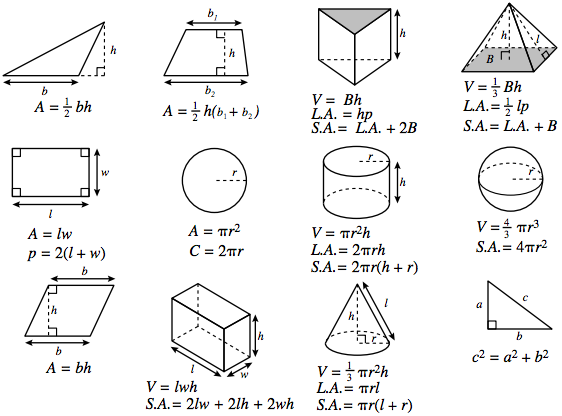
\includegraphics[width=5.5in]{geometric.png}\\


\end{document}
